\documentclass[aspectratio=169,10pt]{beamer}

\usetheme{default}
\usefonttheme{professionalfonts}
\setbeamertemplate{navigation symbols}{}

\usepackage[utf8]{inputenc}
\usepackage[T1]{fontenc}
\usepackage{lmodern}
\usepackage{amsmath,amssymb}
\usepackage{booktabs}
\usepackage{multirow}
\usepackage{graphicx}
\graphicspath{{../}{./}{../figures/}{figures/}}
\usepackage{xcolor}
\usepackage{tikz}
\usepackage{hyperref}

% -----------------------------------------------------------------------------
% Editorial Color Palette (inspired by DEEPL_LEARNING_SLIDES.pdf)
% -----------------------------------------------------------------------------
\definecolor{bgcream}{HTML}{F7F6F2}
\definecolor{textdark}{HTML}{1E1E1E}
\definecolor{textmuted}{HTML}{68645E}
\definecolor{accentbronze}{HTML}{A67244}
\definecolor{rulegray}{HTML}{D6D3CB}
\definecolor{cardbg}{HTML}{FFFFFF}
\definecolor{darkslide}{HTML}{1E1E1E}

\setbeamercolor{background canvas}{bg=bgcream}
\setbeamercolor{normal text}{fg=textdark}
\setbeamercolor{structure}{fg=accentbronze}
\setbeamercolor{frametitle}{fg=textdark,bg=bgcream}
\setbeamercolor{itemize item}{fg=accentbronze}
\setbeamercolor{itemize subitem}{fg=accentbronze}

\setbeamertemplate{itemize item}{\raisebox{0.12ex}{\tikz\fill[accentbronze] (0,0) circle (1.5pt);}}
\setbeamertemplate{itemize subitem}{\raisebox{0.12ex}{\tikz\draw[accentbronze,line width=0.6pt] (0,0) circle (1.3pt);}}

\setbeamersize{text margin left=1.1cm, text margin right=1.1cm}

% Clean Editorial Frame Title
\setbeamertemplate{frametitle}{%
    \vspace{0.38cm}%
    {\rmfamily\fontsize{20}{24}\selectfont\color{textdark}\insertframetitle}%
    \vspace{0.08cm}%
}

% Minimal Footer with proper bottom padding and reserved height
\setbeamertemplate{footline}{%
    \hbox to \paperwidth{%
        \rule[-0.24cm]{0pt}{0.52cm}%
        \ifnum\theframenumber>1
            \ifnum\theframenumber<\inserttotalframenumber
                \hspace{1.1cm}%
                {\fontsize{6.5}{8}\selectfont\color{textmuted}\MakeUppercase{PXP Quantum Dynamics $\cdot$ Gligora \& Lavorato}}%
                \hfill%
                {\fontsize{6.5}{8}\selectfont\color{textmuted}\insertframenumber\ / \inserttotalframenumber}%
                \hspace{1.1cm}%
            \else
                \hfill%
            \fi
        \else
            \hfill%
        \fi
    }%
}

% Helper command for white-framed figure cards with constrained height and italic caption
\newcommand{\figcardh}[4]{%
    \begin{minipage}{#1}
        \setlength{\fboxsep}{4pt}%
        \setlength{\fboxrule}{0.5pt}%
        \fcolorbox{rulegray}{cardbg}{%
            \begin{minipage}{\dimexpr\linewidth-9pt\relax}
                \centering
                \includegraphics[width=\linewidth,height=#2,keepaspectratio]{#3}
            \end{minipage}%
        }\par\vspace{2.5pt}
        {\raggedright\rmfamily\itshape\fontsize{7.5}{9}\selectfont\color{textmuted}#4\par}
    \end{minipage}%
}

\begin{document}

% =============================================================================
% SLIDE 1: Title Slide
% =============================================================================
\begin{frame}[plain]
    \vspace{1.25cm}
    {\fontsize{8}{10}\selectfont\color{accentbronze}\MakeUppercase{Deep Learning $\cdot$ Final Project}}\\[0.45cm]
    {\rmfamily\fontsize{25}{31}\selectfont\color{textdark}Quantum Dynamics: Predicting\\Qubit Evolution with Deep Learning}\\[0.45cm]
    {\color{accentbronze}\rule{4.5cm}{0.7pt}}\\[0.35cm]
    {\fontsize{11.5}{15}\selectfont\color{textdark}Sequence models for PXP quantum dynamics forecasting}\\[0.45cm]
    {\fontsize{8.5}{11.5}\selectfont\color{textmuted}Deep Learning course, Artificial Intelligence and Computer Science --- University of Calabria,\\A.Y.\ 2025/2026}\\[0.45cm]
    {\fontsize{10.5}{13}\selectfont\color{textdark}Ernesto Gligora $\cdot$ Riccardo Lavorato}
\end{frame}

% =============================================================================
% SLIDE 2: Problem & Tasks
% =============================================================================
\begin{frame}{Problem \& Tasks}
    \vspace{0.05cm}
    \begin{itemize}\setlength{\itemsep}{7pt}
        \item \fontsize{10}{13.5}\selectfont \textbf{Goal:} exponentially costly $N=10$ PXP quantum simulation $\rightarrow$ learn a fast data-driven surrogate ($D=55$ observables, $T_{\text{out}}=40$)
        \item \textbf{One leak-free pipeline, two model families:} RNN ($\text{M1}\rightarrow\text{M2}$), Transformer ($\text{M3}\rightarrow\text{M4}$) + Lab~6 Autoencoder pilot
        \item \textbf{Three core challenges} tackled alongside rigorous statistical validation (3 seeds + 5-Fold CV)
    \end{itemize}

    \vspace{0.48cm}
    \begin{columns}[T]
        \begin{column}{0.30\textwidth}
            {\color{rulegray}\rule{\linewidth}{0.6pt}}\\[0.22cm]
            {\fontsize{7.5}{9}\selectfont\color{accentbronze}\MakeUppercase{Challenge 01}}\\[0.15cm]
            {\rmfamily\fontsize{14}{17}\selectfont\color{textdark}Input window}\\[0.1cm]
            {\fontsize{8.8}{11.5}\selectfont\color{textmuted}Minimize $T_{\text{in}} \in \{5,10,20,40\}$ on strictly aligned targets}
        \end{column}
        \begin{column}{0.30\textwidth}
            {\color{rulegray}\rule{\linewidth}{0.6pt}}\\[0.22cm]
            {\fontsize{7.5}{9}\selectfont\color{accentbronze}\MakeUppercase{Challenge 02}}\\[0.15cm]
            {\rmfamily\fontsize{14}{17}\selectfont\color{textdark}Super-resolution}\\[0.1cm]
            {\fontsize{8.8}{11.5}\selectfont\color{textmuted}Reconstruct native $\Delta t = 0.02\text{ s}$ from $2\times$ coarser input}
        \end{column}
        \begin{column}{0.30\textwidth}
            {\color{rulegray}\rule{\linewidth}{0.6pt}}\\[0.22cm]
            {\fontsize{7.5}{9}\selectfont\color{accentbronze}\MakeUppercase{Challenge 03}}\\[0.15cm]
            {\rmfamily\fontsize{14}{17}\selectfont\color{textdark}Interpretability}\\[0.1cm]
            {\fontsize{8.8}{11.5}\selectfont\color{textmuted}Explain physical dynamics via multi-head attention maps}
        \end{column}
    \end{columns}
\end{frame}

% =============================================================================
% SLIDE 3: Dataset & Preprocessing
% =============================================================================
\begin{frame}{Dataset \& Preprocessing}
    \begin{columns}[T]
        \begin{column}{0.43\textwidth}
            {\rmfamily\fontsize{12}{14}\selectfont\color{textdark}Data}\\[0.06cm]
            \begin{itemize}\setlength{\itemsep}{2.5pt}
                \item \fontsize{8.6}{11}\selectfont PXP, $N=10$ qubits, $400$ trajectories, $\Delta t=0.02\text{ s}$
                \item $55$ features: $10$ magnetizations $\langle\sigma_z^i\rangle + 45$ correlations $\langle\sigma_z^i\sigma_z^j\rangle$
                \item Bounded $[-1,1]$ ($0\%$ violations) $\rightarrow$ $\tanh$ head, no normalization (\texttt{none}: $2.17\text{e-}4$ vs.\ Z-score: $2.32\text{e-}4$)
            \end{itemize}

            \vspace{0.12cm}
            {\rmfamily\fontsize{12}{14}\selectfont\color{textdark}Setup}\\[0.06cm]
            \begin{itemize}\setlength{\itemsep}{2.5pt}
                \item \fontsize{8.6}{11}\selectfont Split per trajectory: $280 / 60 / 60$, $\texttt{seed}=42$
                \item Windows: $\texttt{short}=10$ / $\texttt{long}=20$, $\texttt{output}=40$, $\texttt{stride}=10$
                \item Aligned targets ($\texttt{align\_t\_in}=40$) for Challenge~1
            \end{itemize}
        \end{column}
        \begin{column}{0.53\textwidth}
            \centering
            \figcardh{0.96\linewidth}{2.2cm}{figures/02_windowing/tin_grid_comparison.jpeg}{Sliding-window extraction with strictly aligned future targets ($t_0 = 0.80\text{ s}$)}\\[0.1cm]
            \figcardh{0.96\linewidth}{2.05cm}{figures/01_data/normalization_loss_curves.jpeg}{Normalization ablation: raw physical scale (\texttt{none} + $\tanh$) vs.\ Z-score}
        \end{column}
    \end{columns}
\end{frame}

% =============================================================================
% SLIDE 4: Model Roadmap
% =============================================================================
\begin{frame}{Model Roadmap}
    \vspace{0.02cm}
    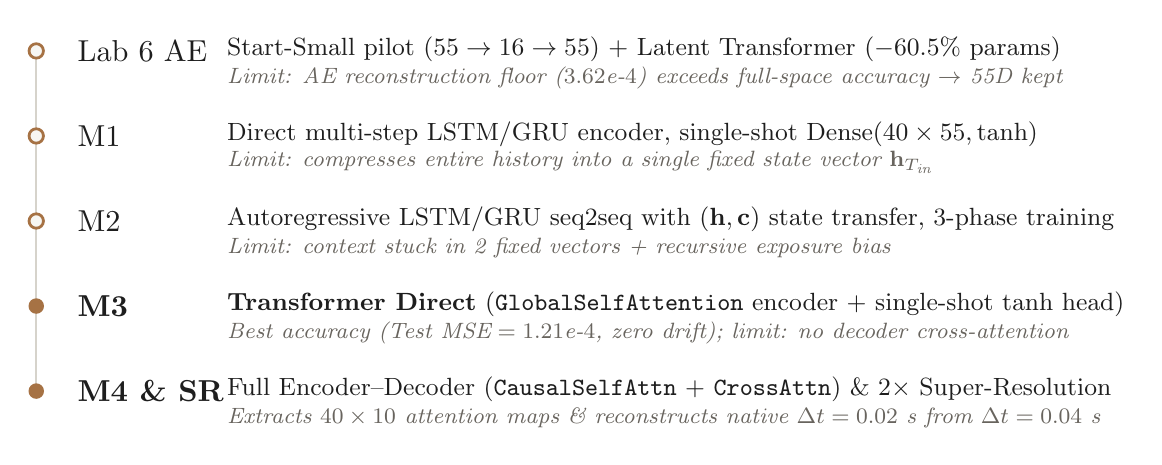
\begin{tikzpicture}[x=1cm,y=1cm]
        % Vertical timeline line
        \draw[rulegray, line width=0.8pt] (0, 0.05) -- (0, -4.35);

        % Node 1: Pilot AE
        \fill[bgcream] (0, 0) circle (2.6pt);
        \draw[accentbronze, line width=1pt] (0, 0) circle (2.6pt);
        \node[anchor=west, font=\rmfamily\fontsize{11}{13}\selectfont, text=textdark] at (0.4, 0) {Lab~6 AE};
        \node[anchor=west, font=\fontsize{9}{11.5}\selectfont, text=textdark] at (2.3, 0.02) {Start-Small pilot ($55\rightarrow 16\rightarrow 55$) + Latent Transformer ($-60.5\%$ params)};
        \node[anchor=west, font=\rmfamily\itshape\fontsize{8}{10}\selectfont, text=textmuted] at (2.3, -0.34) {Limit: AE reconstruction floor ($3.62\text{e-}4$) exceeds full-space accuracy $\rightarrow$ 55D kept};

        % Node 2: M1
        \fill[bgcream] (0, -1.08) circle (2.6pt);
        \draw[accentbronze, line width=1pt] (0, -1.08) circle (2.6pt);
        \node[anchor=west, font=\rmfamily\fontsize{11}{13}\selectfont, text=textdark] at (0.4, -1.08) {M1};
        \node[anchor=west, font=\fontsize{9}{11.5}\selectfont, text=textdark] at (2.3, -1.06) {Direct multi-step LSTM/GRU encoder, single-shot $\text{Dense}(40\times 55, \tanh)$};
        \node[anchor=west, font=\rmfamily\itshape\fontsize{8}{10}\selectfont, text=textmuted] at (2.3, -1.42) {Limit: compresses entire history into a single fixed state vector $\mathbf{h}_{T_{\text{in}}}$};

        % Node 3: M2
        \fill[bgcream] (0, -2.16) circle (2.6pt);
        \draw[accentbronze, line width=1pt] (0, -2.16) circle (2.6pt);
        \node[anchor=west, font=\rmfamily\fontsize{11}{13}\selectfont, text=textdark] at (0.4, -2.16) {M2};
        \node[anchor=west, font=\fontsize{9}{11.5}\selectfont, text=textdark] at (2.3, -2.14) {Autoregressive LSTM/GRU seq2seq with $(\mathbf{h},\mathbf{c})$ state transfer, 3-phase training};
        \node[anchor=west, font=\rmfamily\itshape\fontsize{8}{10}\selectfont, text=textmuted] at (2.3, -2.50) {Limit: context stuck in 2 fixed vectors + recursive exposure bias};

        % Node 4: M3
        \fill[accentbronze] (0, -3.24) circle (2.8pt);
        \node[anchor=west, font=\rmfamily\fontsize{11}{13}\selectfont, text=textdark] at (0.4, -3.24) {\textbf{M3}};
        \node[anchor=west, font=\fontsize{9}{11.5}\selectfont, text=textdark] at (2.3, -3.22) {\textbf{Transformer Direct} (\texttt{GlobalSelfAttention} encoder + single-shot $\tanh$ head)};
        \node[anchor=west, font=\rmfamily\itshape\fontsize{8}{10}\selectfont, text=textmuted] at (2.3, -3.58) {Best accuracy ($\text{Test MSE} = 1.21\text{e-}4$, zero drift); limit: no decoder cross-attention};

        % Node 5: M4 & SR
        \fill[accentbronze] (0, -4.32) circle (2.8pt);
        \node[anchor=west, font=\rmfamily\fontsize{11}{13}\selectfont, text=textdark] at (0.4, -4.32) {\textbf{M4 \& SR}};
        \node[anchor=west, font=\fontsize{9}{11.5}\selectfont, text=textdark] at (2.3, -4.30) {Full Encoder--Decoder (\texttt{CausalSelfAttn} + \texttt{CrossAttn}) \& $2\times$ Super-Resolution};
        \node[anchor=west, font=\rmfamily\itshape\fontsize{8}{10}\selectfont, text=textmuted] at (2.3, -4.66) {Extracts $40\times 10$ attention maps \& reconstructs native $\Delta t=0.02\text{ s}$ from $\Delta t=0.04\text{ s}$};
    \end{tikzpicture}
\end{frame}

% =============================================================================
% SLIDE 5: Training Curriculum
% =============================================================================
\begin{frame}{Training Curriculum}
    \begin{columns}[T]
        \begin{column}{0.45\textwidth}
            \begin{itemize}\setlength{\itemsep}{6pt}
                \item \fontsize{9}{12}\selectfont $\text{Teacher Forcing (10)} \rightarrow \text{Masked Modeling (10)} \rightarrow \text{Scheduled Sampling (5)} = 25\text{ epochs}$
                \item \textbf{Direct models (M1, M3):} random $15\%$ timestep masking ($p_{\text{mask}}=0.15$) forces non-local context interpolation
                \item \textbf{Seq2Seq models (M2, M4):} two-pass Scheduled Sampling ($p: 0.0 \rightarrow 0.5$) mitigates open-loop recursive drift
            \end{itemize}

            \vspace{0.18cm}
            {\color{rulegray}\rule{\linewidth}{0.6pt}}\\[0.12cm]
            \begin{columns}[T]
                \begin{column}{0.31\linewidth}
                    {\rmfamily\fontsize{16}{19}\selectfont\color{accentbronze}10}\\[2pt]
                    {\fontsize{7.8}{9.5}\selectfont\color{textdark}Teacher\\Forcing}
                \end{column}
                \begin{column}{0.31\linewidth}
                    {\rmfamily\fontsize{16}{19}\selectfont\color{accentbronze}10}\\[2pt]
                    {\fontsize{7.8}{9.5}\selectfont\color{textdark}Masked\\Modeling}
                \end{column}
                \begin{column}{0.31\linewidth}
                    {\rmfamily\fontsize{16}{19}\selectfont\color{accentbronze}5}\\[2pt]
                    {\fontsize{7.8}{9.5}\selectfont\color{textdark}Scheduled\\Sampling}
                \end{column}
            \end{columns}
            \vspace{0.10cm}
            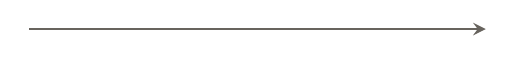
\begin{tikzpicture}
                \draw[->, >=stealth, color=textmuted, line width=1.0pt] (0,0) -- (5.8,0);
            \end{tikzpicture}
        \end{column}
        \begin{column}{0.52\textwidth}
            \centering
            \figcardh{0.96\linewidth}{2.2cm}{figures/04_transformer/loss_curves_hybrid.jpeg}{Validation MSE across the 3-phase curriculum (M3 Direct vs.\ M4 Seq2Seq)}\\[0.12cm]
            \figcardh{0.96\linewidth}{2.2cm}{figures/04_transformer/free_running_error_accumulation.jpeg}{Step-by-step error propagation: Teacher Forcing vs.\ Free-Running vs.\ One-Shot M3}
        \end{column}
    \end{columns}
\end{frame}

% =============================================================================
% SLIDE 6: Hyperparameter Tuning
% =============================================================================
\begin{frame}{Hyperparameter Tuning}
    \begin{itemize}\setlength{\itemsep}{4pt}
        \item \fontsize{9.2}{12.5}\selectfont Full grid evaluation: $3\text{ configs (HP1, HP2, HP3)} \times 2\text{ windows (\texttt{short}, \texttt{long})} \times 4\text{ architectures} = 24\text{ models}$
        \item Multi-seed stability ($\texttt{seeds } 42, 43, 44$) + $5$-Fold Trajectory Cross-Validation ($340$ trajectories) on top winners
    \end{itemize}

    \vspace{0.28cm}
    \begin{columns}[T]
        \begin{column}{0.46\textwidth}
            \setlength{\fboxsep}{9pt}%
            \setlength{\fboxrule}{0.5pt}%
            \fcolorbox{rulegray}{cardbg}{%
                \begin{minipage}{\dimexpr\linewidth-19pt\relax}
                    {\fontsize{7.5}{9}\selectfont\color{accentbronze}\MakeUppercase{M1 / M2 (RNN Winner --- HP1 / HP2)}}\\[0.22cm]
                    \footnotesize
                    \begin{tabular*}{\linewidth}{@{\extracolsep{\fill}}lr@{}}
                        \texttt{cell\_type} & \textbf{LSTM} \\
                        \specialrule{0.4pt}{3.5pt}{3.5pt}
                        \texttt{rnn\_units} & \textbf{64} \\
                        \specialrule{0.4pt}{3.5pt}{3.5pt}
                        \texttt{num\_layers} & \textbf{1 (M1) / 2 (M2)} \\
                        \specialrule{0.4pt}{3.5pt}{3.5pt}
                        \texttt{dropout} & \textbf{0.0 (M1) / 0.10 (M2)} \\
                        \specialrule{0.4pt}{3.5pt}{3.5pt}
                        \texttt{lr (Adam)} & \textbf{0.001} \\
                    \end{tabular*}
                \end{minipage}%
            }
        \end{column}
        \begin{column}{0.46\textwidth}
            \setlength{\fboxsep}{9pt}%
            \setlength{\fboxrule}{0.5pt}%
            \fcolorbox{rulegray}{cardbg}{%
                \begin{minipage}{\dimexpr\linewidth-19pt\relax}
                    {\fontsize{7.5}{9}\selectfont\color{accentbronze}\MakeUppercase{M3 / M4 (Transformer Winner --- HP3 / HP1)}}\\[0.22cm]
                    \footnotesize
                    \begin{tabular*}{\linewidth}{@{\extracolsep{\fill}}lr@{}}
                        \texttt{d\_model} & \textbf{64} \\
                        \specialrule{0.4pt}{3.5pt}{3.5pt}
                        \texttt{num\_heads} & \textbf{2 (M3) / 4 (M4)} \\
                        \specialrule{0.4pt}{3.5pt}{3.5pt}
                        \texttt{num\_layers (blocks)} & \textbf{1 (M3) / 2 (M4)} \\
                        \specialrule{0.4pt}{3.5pt}{3.5pt}
                        \texttt{ff\_dim} & $\mathbf{2 \cdot d_{\text{model}} = 128}$ \\
                        \specialrule{0.4pt}{3.5pt}{3.5pt}
                        \texttt{lr (Adam)} & \textbf{0.001} \\
                    \end{tabular*}
                \end{minipage}%
            }
        \end{column}
    \end{columns}
\end{frame}

% =============================================================================
% SLIDE 7: Test Set Performance, Short & Long Windows
% =============================================================================
\begin{frame}{Test Set Performance \& Statistical Validation}
    {\fontsize{8.5}{11}\selectfont\color{textmuted}Mean $\pm$ CI95\% over 3 seeds (42/43/44) and 5-Fold CV on \texttt{short} ($T_{\text{in}}=10$). Best per column in \textbf{bold}.}

    \vspace{0.3cm}
    \renewcommand{\arraystretch}{1.5}
    \resizebox{\textwidth}{!}{%
    \begin{tabular}{lcccc}
        {\fontsize{7.5}{9}\selectfont\color{textmuted}MODEL} &
        {\fontsize{7.5}{9}\selectfont\color{textmuted}3-SEED VAL MSE (SHORT)} &
        {\fontsize{7.5}{9}\selectfont\color{textmuted}5-FOLD CV MSE} &
        {\fontsize{7.5}{9}\selectfont\color{textmuted}TEST MSE (SHORT / LONG)} &
        {\fontsize{7.5}{9}\selectfont\color{textmuted}INFERENCE MODE / GAP} \\
        \toprule[0.8pt]
        Persistence Baseline & $6.21\text{e-}4$ & --- & $6.23\text{e-}4$ / $6.21\text{e-}4$ & \textcolor{textmuted}{n/a} \\
        \specialrule{0.3pt}{0pt}{0pt}
        M1 (LSTM direct, HP1) & $1.61\text{e-}4 \pm 1.3\text{e-}6$ & $1.60\text{e-}4 \pm 2.1\text{e-}6$ & $1.61\text{e-}4$ / $1.47\text{e-}4$ & \textcolor{textmuted}{one-shot (no drift)} \\
        \specialrule{0.3pt}{0pt}{0pt}
        M2 (LSTM seq2seq, HP2) & $2.66\text{e-}4 \pm 5.0\text{e-}6$ & --- & $2.66\text{e-}4$ / $2.42\text{e-}4$ & $2.66\text{e-}4$ (AR rollout) \\
        \specialrule{0.3pt}{0pt}{0pt}
        \textbf{M3 (Transformer direct, HP3)} & $\mathbf{1.21\text{e-}4 \pm 1.0\text{e-}6}$ & $\mathbf{1.20\text{e-}4 \pm 2.3\text{e-}6}$ & $\mathbf{1.21\text{e-}4}$ / $\mathbf{1.21\text{e-}4}$ & \textbf{one-shot ($\mathbf{-25\%}$ vs.\ M1)} \\
        \specialrule{0.3pt}{0pt}{0pt}
        M4 (Transformer seq2seq, HP1) & $4.02\text{e-}4 \pm 1.3\text{e-}5$ & --- & $3.96\text{e-}4$ / $3.38\text{e-}4$ & TF $\mathbf{7.80\text{e-}5} \rightarrow$ FR $3.96\text{e-}4$ \\
        \bottomrule[0.6pt]
    \end{tabular}%
    }

    \vspace{0.32cm}
    {\fontsize{9}{12}\selectfont\color{textdark}\textbf{Key result:} One-shot \textbf{M3} eliminates recursive exposure bias, reducing global MSE by $\mathbf{25\%}$ and single-qubit magnetization MSE by $\mathbf{50\%}$ ($3.60\text{e-}5$ vs.\ $7.20\text{e-}5$) over the best RNN.}
\end{frame}

% =============================================================================
% SLIDE 8: Challenge 1: Minimal Input Window
% =============================================================================
\begin{frame}{Challenge 1: Minimal Input Window}
    \begin{itemize}\setlength{\itemsep}{3pt}
        \item \fontsize{8.8}{11.5}\selectfont Evaluated across $T_{\text{in}} \in \{5, 10, 20, 40\}$ on \textbf{strictly aligned targets} ($\texttt{align\_t\_in}=40$, same $5,580$ test segments)
        \item \textbf{M1 (LSTM):} improves from $T_{\text{in}}=5$ ($1.72\text{e-}4$) to $T_{\text{in}}=20$ ($1.48\text{e-}4$), then \textbf{saturates completely} at $T_{\text{in}}=40$ ($1.48\text{e-}4$)
        \item \textbf{M3 (Transformer):} beats the best LSTM even at $T_{\text{in}}=5$ ($1.23\text{e-}4$) and scales to $\mathbf{1.11\text{e-}4}$ at $T_{\text{in}}=40$ ($-9\%$)
    \end{itemize}

    \vspace{0.10cm}
    \begin{columns}[T]
        \begin{column}{0.48\textwidth}
            \centering
            \figcardh{0.98\linewidth}{2.75cm}{figures/04_transformer/challenge1_tin_scaling.jpeg}{Aligned-target MSE scaling across $T_{\text{in}} \in \{5, 10, 20, 40\}$ for M3 Transformer}
        \end{column}
        \begin{column}{0.48\textwidth}
            \centering
            \figcardh{0.98\linewidth}{2.75cm}{figures/05_inference/global_benchmark_summary.jpeg}{Validation MSE comparison across all four model families (short vs.\ long window)}
        \end{column}
    \end{columns}
\end{frame}

% =============================================================================
% SLIDE 9: Challenge 2: Super-Resolution
% =============================================================================
\begin{frame}{Challenge 2: Super-Resolution}
    \begin{columns}[T]
        \begin{column}{0.41\textwidth}
            \vspace{0.15cm}
            \begin{itemize}\setlength{\itemsep}{7pt}
                \item \fontsize{9}{12.2}\selectfont \textbf{Test MSE $\mathbf{1.21\text{e-}4}$} ($\text{MAE } 0.00788$) from $2\times$ coarser input ($20$ steps at $\Delta t_{\text{sub}} = 0.04\text{ s}$)
                \item \textbf{Matches standard M3} ($1.21\text{e-}4$) and sits within $\Delta\text{MSE} = 1.1\text{e-}5$ of dense 39-step native M3 ($1.10\text{e-}4$)
                \item \textbf{No architecture change:} $f_{\text{Nyq}} = 12.5\text{ Hz} \gg f_{\text{scar}} \approx 0.7\text{ Hz}$ allows exact PXP phase recovery
            \end{itemize}
        \end{column}
        \begin{column}{0.55\textwidth}
            \centering
            \figcardh{0.98\linewidth}{2.75cm}{figures/04_transformer/challenge2_super_resolution.jpeg}{M3-SR reconstruction of a $2\times$ subsampled test trajectory and horizon error profile}\\[0.22cm]
            \setlength{\fboxsep}{7pt}%
            \setlength{\fboxrule}{0.5pt}%
            \fcolorbox{rulegray}{cardbg}{%
                \begin{minipage}{\dimexpr0.98\linewidth-15pt\relax}
                    {\fontsize{7}{8.5}\selectfont\color{accentbronze}\MakeUppercase{Super-Resolution vs.\ Native Sampling (Aligned Targets)}}\\[4pt]
                    \scriptsize\setlength{\tabcolsep}{2.5pt}%
                    \begin{tabular*}{\linewidth}{@{\extracolsep{\fill}}lccc@{}}
                        \textbf{Setting} & $\Delta t_{\text{in}}$ & \textbf{Test MSE} & \textbf{Test MAE} \\
                        \specialrule{0.4pt}{2pt}{2pt}
                        \textbf{M3-SR ($\times 2$, 20 pts)} & $\mathbf{0.04\text{ s}}$ & $\mathbf{1.21\text{e-}4}$ & $\mathbf{0.00788}$ \\
                        M3 Native (39 pts) & $0.02\text{ s}$ & $1.10\text{e-}4$ & $0.00754$ \\
                        M3 Standard \texttt{short} (10 pts) & $0.02\text{ s}$ & $1.21\text{e-}4$ & $0.00785$ \\
                    \end{tabular*}
                \end{minipage}%
            }
        \end{column}
    \end{columns}
\end{frame}

% =============================================================================
% SLIDE 10: Challenge 3: Attention Maps
% =============================================================================
\begin{frame}{Challenge 3: Attention Maps}
    \begin{columns}[T]
        \begin{column}{0.41\textwidth}
            \vspace{0.15cm}
            \begin{itemize}\setlength{\itemsep}{7pt}
                \item \fontsize{9}{12.2}\selectfont \textbf{Heads 1 \& 4 (Boundary Anchoring):} cross-attention concentrates on final input steps $t \in [-0.04, 0.00]\text{ s}$ to lock initial state and slope
                \item \textbf{Heads 2 \& 3 (Quantum-Scar Memory):} non-local attention bands across earlier lags track PXP revival frequency
                \item \textbf{Strict Causal Mask ($40\times 40$):} upper triangle $\max_{j>i}|\alpha_{ij}| = \mathbf{0.00}$ (zero future leakage)
            \end{itemize}
        \end{column}
        \begin{column}{0.55\textwidth}
            \centering
            \figcardh{0.98\linewidth}{2.15cm}{figures/04_transformer/challenge3_cross_attention_heads.jpeg}{M4 decoder cross-attention across all 4 heads ($40$ future queries $\times 10$ past keys)}\\[0.12cm]
            \figcardh{0.98\linewidth}{2.25cm}{figures/04_transformer/challenge3_causal_mask_verification.jpeg}{Decoder lower-triangular causal mask ($40\times 40$) and encoder bidirectional self-attention}
        \end{column}
    \end{columns}
\end{frame}

% =============================================================================
% SLIDE 11: Blind Test Forecast & Disaggregated Analysis
% =============================================================================
\begin{frame}{Blind Test Forecast \& Physical Analysis}
    \begin{columns}[T]
        \begin{column}{0.48\textwidth}
            \centering
            \figcardh{0.98\linewidth}{2.95cm}{figures/05_inference/test_set_live_prediction.jpeg}{Forecast comparison on blind test Trajectory \#6 ($m_1$ and $c_{1,2}$), M1 RNN vs.\ M3 Transformer}
        \end{column}
        \begin{column}{0.48\textwidth}
            \centering
            \figcardh{0.98\linewidth}{2.95cm}{figures/04_transformer/disaggregated_error_analysis.jpeg}{Disaggregated physical error: per-qubit magnetization MSE, $c_{ij}$ matrix, and horizon drift}
        \end{column}
    \end{columns}

    \vspace{0.18cm}
    \begin{itemize}\setlength{\itemsep}{3pt}
        \item \fontsize{8.8}{11.5}\selectfont \textbf{M3 vs.\ M1 on Blind Test ($5,760$ windows in $1.72\text{ s}$):} M3 tracks turning points of $m_1(t)$ and $c_{1,2}(t)$ with superior phase fidelity
        \item \textbf{Boundary vs.\ Bulk Qubits:} edge qubits ($q_1, q_{10}$) achieve lower MSE than central bulk qubits ($q_5, q_6$) due to open-chain boundary reflection
        \item \textbf{Physical Consistency:} $100\%$ of test predictions satisfy two-body quantum positivity ($\min P(s_i,s_j) = \mathbf{0.1632 > 0}$)
    \end{itemize}
\end{frame}

% =============================================================================
% SLIDE 12: Future Work
% =============================================================================
\begin{frame}{Future Work}
    \vspace{0.55cm}
    \begin{columns}[T]
        \begin{column}{0.30\textwidth}
            {\color{rulegray}\rule{\linewidth}{0.6pt}}\\[0.32cm]
            {\rmfamily\fontsize{22}{26}\selectfont\color{accentbronze}01}\\[0.28cm]
            {\rmfamily\fontsize{14}{17}\selectfont\color{textdark}Longer horizon}\\[0.14cm]
            {\fontsize{8.8}{12}\selectfont\color{textmuted}Chain 40-step M3 blocks in block-autoregressive rollouts to extend $T_{\text{out}} \ge 160$ with $40\times$ fewer feedback steps}
        \end{column}
        \begin{column}{0.30\textwidth}
            {\color{rulegray}\rule{\linewidth}{0.6pt}}\\[0.32cm]
            {\rmfamily\fontsize{22}{26}\selectfont\color{accentbronze}02}\\[0.28cm]
            {\rmfamily\fontsize{14}{17}\selectfont\color{textdark}Coarser super-resolution}\\[0.14cm]
            {\fontsize{8.8}{12}\selectfont\color{textmuted}Test $4\times$ and $8\times$ subsampling limits ($\Delta t_{\text{sub}} \in \{0.08, 0.16\}\text{ s}$) to locate the empirical Nyquist breakdown of PXP scars}
        \end{column}
        \begin{column}{0.30\textwidth}
            {\color{rulegray}\rule{\linewidth}{0.6pt}}\\[0.32cm]
            {\rmfamily\fontsize{22}{26}\selectfont\color{accentbronze}03}\\[0.28cm]
            {\rmfamily\fontsize{14}{17}\selectfont\color{textdark}Larger qubit systems}\\[0.14cm]
            {\fontsize{8.8}{12}\selectfont\color{textmuted}Replace the fixed 55D projection with a spatial Graph-Attention encoder over the Rydberg chain to scale past $N=10$}
        \end{column}
    \end{columns}
\end{frame}

% =============================================================================
% SLIDE 13: Closing Slide
% =============================================================================
{
\setbeamercolor{background canvas}{bg=darkslide}
\begin{frame}[plain]
    \vspace{2.1cm}
    {\rmfamily\fontsize{30}{36}\selectfont\color{white}Thank you --- Questions?}\par\vspace{0.42cm}
    {\color{accentbronze}\rule{3.8cm}{0.7pt}}\par\vspace{0.38cm}
    {\fontsize{10.5}{13}\selectfont\color{white}Ernesto Gligora $\cdot$ Riccardo Lavorato}\par\vspace{0.18cm}
    {\fontsize{8.5}{11}\selectfont\color{rulegray}University of Calabria --- A.Y.\ 2025/2026 $\quad\cdot\quad$ \url{https://github.com/Riccardo-27/DL-Quantum}}
\end{frame}
}

\end{document}
